\chapter{Definizione dell'architettura software}

\section{Introduzione}
In questa sezione procederemo a definire l'architettura software della piattaforma.

Data la natura dell'applicazione, i casi d'uso individuati e le feature che il sistema dovrà offrire, è stato deciso di sviluppare una web app, accessibile sia da desktop che da mobile (responsive), in maniera da permettere all'intero team di sviluppo di :
\begin{itemize}
    \item segnalare comodamente i bug da un'interfaccia desktop, inserendo delle descrizioni approfondite
    \item monitorare lo stato delle diverse segnalazioni, sia da desktop che da mobile, avendo a disposizione molte segnalazioni nella stessa  schermata nella versione desktop, ma anche visualizzarne una nel dettaglio tramite l'interfaccia mobile
    \item garantire la sincronizzazione e la centralizzazione dei dati, indipendentemente dal dispositivo utilizzato per l'accesso
\end{itemize}

\section{Architettura Logica}
In conformità con i requisiti non funzionali e i vincoli di progetto, l'architettura di \textit{BugBoard26} è di tipo distribuito, basata sul paradigma Client-Server e sullo stile architetturale \textit{REpresentational State Transfer} (REST).

Il sistema è decomposto in due macro-componenti logicamente e fisicamente separati, che comunicano esclusivamente tramite protocollo HTTP scambiando messaggi in formato JSON:

\begin{itemize}
    \item \textbf{Frontend (Client):} Responsabile della logica di presentazione e dell'interazione utente. Implementato come \textit{Single Page Application} (SPA), questo modulo è completamente disaccoppiato dal backend, garantendo la possibilità di evoluzione indipendente o la sostituzione dell'interfaccia senza impatti sulla logica di business.
    \item \textbf{Backend (Server):} Responsabile della logica di business, della sicurezza e della persistenza dei dati. Il backend espone interfacce di programmazione (API) pubbliche e opera in modalità \textit{stateless}: ogni richiesta contiene tutte le informazioni necessarie per essere elaborata, garantendo la scalabilità orizzontale.
\end{itemize}

\section{Pattern Architetturale Backend}
Il modulo Backend è strutturato internamente secondo il pattern \textbf{Layered Architecture} (Architettura a Strati) per garantire la \textit{Separation of Concerns}. Il flusso di elaborazione di una richiesta attraversa i seguenti livelli:

\begin{itemize}
    \item \textbf{Interface Layer (Controller):} Punto di ingresso delle richieste REST. Gestisce la validazione sintattica degli input (DTO) e la mappatura delle risposte HTTP.
    \item \textbf{Business Logic Layer (Service):} Implementa le regole di dominio, i controlli di sicurezza applicativa e il coordinamento delle transazioni. È isolato dai dettagli dell'interfaccia utente e della persistenza.
    \item \textbf{Data Access Layer (Repository):} Astrae l'accesso al database relazionale tramite un'interfaccia. Fornisce i metodi per la persistenza e il recupero delle entità, disaccoppiando la logica di business dal linguaggio SQL specifico.
\end{itemize}


\section{Stack tecnologico backend}

\begin{longtable}{|p{4cm}|p{4cm}|p{7cm}|}
    \hline
    \textbf{Componente} & \textbf{Tecnologia Utilizzata} & \textbf{Motivazione} \\
    \hline
    \textbf{Linguaggio Backend}              & Java                                   & Linguaggio fortemente tipizzato, Object-Oriented, utilizzato dal 99\% delle aziende \cite{java-adoption-rate}   \\
    \hline
    \textbf{Framework Backend}               & Spring Boot 4                          & Offre Dependency Injection, semplifica la scrittura del codice rispetto a Java Spring \\
    \hline
    \textbf{Database}                        & PostgresSQL                            & DBMS relazionale robusto, affidabile, sicuro, open source e veloce \\
    \hline
    \textbf{Object-Relational Mapping (ORM)} & Spring Data JPA & Astrazione necessaria per la gestione della persistenza orientata agli oggetti, riducendo il codice boilerplate e prevenendo nativamente SQL Injection                                                                                   \\
    \hline
    \textbf{Container}                       & Docker                                 & Ambiente indipendente che garantisce un funzionamento coerente su ogni ambiente                                                                  \\
    \hline
\end{longtable}

\section{Pattern Architetturale Frontend}
QUESTA PARTE è DA REVISIONARE!!!!!!!!!!!!!!!!!!!!!!!!
Il modulo Frontend è progettato come una \textit{Single Page Application} (SPA) basata su una \textbf{Component-Based Architecture}. L'interfaccia utente è decomposta in unità funzionali indipendenti e riutilizzabili (Componenti), organizzate in una struttura gerarchica ad albero.

Per garantire la manutenibilità e la testabilità del codice client, viene applicata la separazione tra:
\begin{itemize}
    \item \textbf{Container Components (Smart):} Responsabili del recupero dei dati, della gestione dello stato della vista e dell'interazione con i Service di comunicazione.
    \item \textbf{Presentational Components (Dumb):} Responsabili esclusivamente del rendering grafico e dell'intercettazione degli eventi utente, privi di dipendenze dalla logica di business o dai servizi esterni.
\end{itemize}

\paragraph{Gestione della Comunicazione Asincrona}
L'interazione con le API REST del Backend è gestita secondo il \textbf{Observer Pattern}. Utilizzando la libreria \textit{RxJS}, le risposte HTTP sono trattate come flussi di dati (\textit{Streams}) asincroni. Questo approccio reattivo permette all'interfaccia di aggiornarsi dinamicamente al variare dello stato dei dati senza bloccare l'interazione utente, migliorando la percezione di fluidità e performance del sistema.

\section{Dettaglio Tecnologie Frontend}
A integrazione della Tabella \ref{tab:tech_stack}, si motivano le scelte specifiche per il livello di presentazione:

\begin{itemize}
    \item \textbf{Framework: Angular (v17+).} La scelta è motivata dalla natura \textit{strongly-typed} offerta da TypeScript, che garantisce coerenza con il backend Java e riduce gli errori a runtime. Il sistema di \textit{Dependency Injection} nativo di Angular facilita il testing unitario dei componenti e dei servizi di comunicazione.
    \item \textbf{Styling: SCSS e Angular Material.} L'adozione di SCSS permette l'uso di variabili e mixin per mantenere un design system coerente. La libreria di componenti \textit{Angular Material} assicura il rispetto delle linee guida di usabilità e accessibilità (WCAG) con un minimo sforzo implementativo.
\end{itemize}

\section{Architettura Fisica e Deployment}
L'infrastruttura di \textbf{BugBoard26} è interamente ospitata su una piattaforma di cloud computing (come, ad esempio, AWS) per garantire un accesso continuo e universale al sistema. Il deployment si basa sulla containerizzazione tramite \textbf{Docker}, che fornisce un ambiente di esecuzione isolato e indipendente, garantendo un funzionamento coerente dell'applicativo su qualsiasi ambiente hardware o virtuale sottostante.

Fisicamente, il deployment si articola nei seguenti nodi e ambienti di esecuzione:

\begin{description}
    \item[Nodo Cloud - Application Server (Backend):] All'interno dell'infrastruttura cloud, uno o più container Docker sono dedicati all'esecuzione del modulo applicativo sviluppato in Java e basato sul framework \textit{Spring Boot 4}.
    
    \item[Nodo Cloud - Database Server:] Un container Docker ospita il DBMS relazionale \textit{PostgreSQL}, impiegato per la persistenza dei dati. Il backend comunica fisicamente con questo nodo sfruttando l'astrazione ORM fornita da \textit{Spring Data JPA}.
    
    \item[Nodi Client (Dispositivi Utente):] L'accesso al sistema avviene tramite i dispositivi hardware fisici (desktop o mobile) utilizzati dal team. L'ambiente di esecuzione su questi nodi è costituito da un browser web.
    Sul browser viene scaricata ed eseguita l'interfaccia grafica sviluppata in \textit{Angular} e stilizzata tramite SCSS e \textit{Angular Material}.
\end{description}


\section{Descrizione dello schema per la persistenza dati}
\begin{figure}[H]
  \centering
  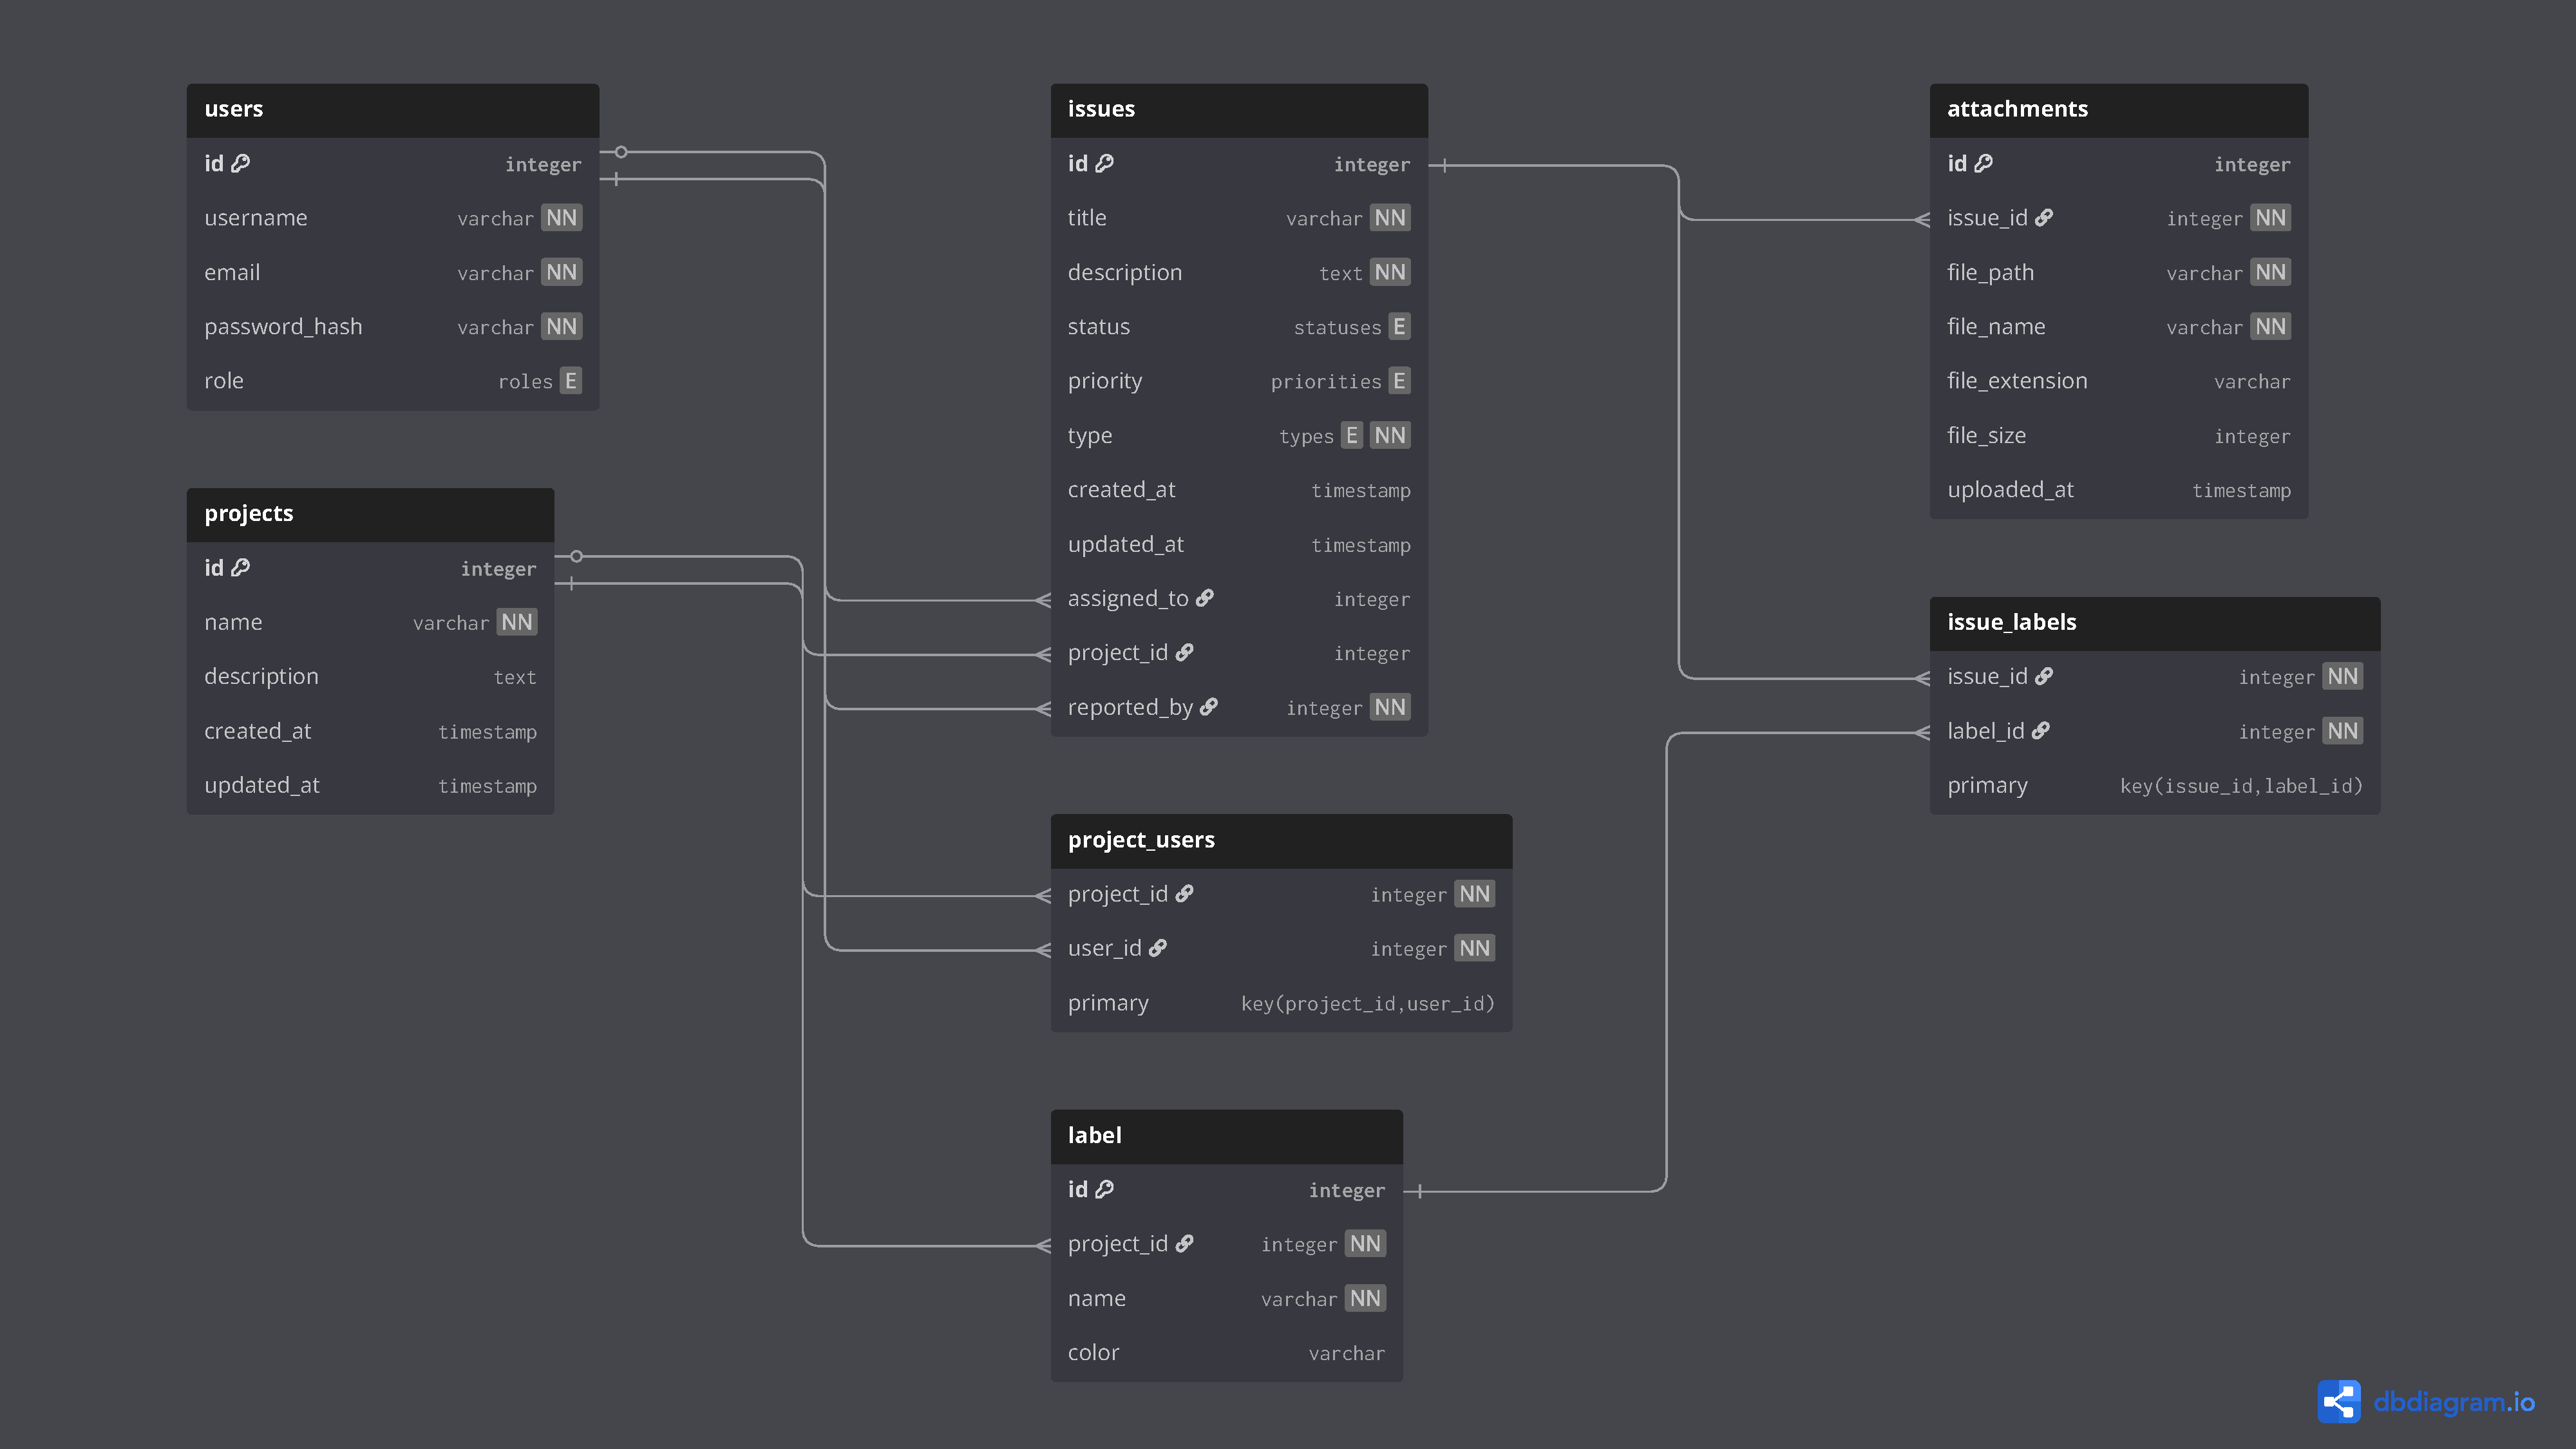
\includegraphics[width=\linewidth,height=0.75\textheight,keepaspectratio]{media/diagrams/database.pdf}
  \caption{Schema di persistenza dei dati}
\end{figure}